\chapter{Prototype}
\label{chap:prototype}

\begin{chapterintro}

In this chapter, we will describe the prototype we developed following the architecture described in the previous chapter. We will start with a short overview of the implemented modules for the system, to then take a detailed look to each one of them, describing how they work, and how they connect to each other.
 
\end{chapterintro}

\cleardoublepage

\section{Overview of the system}

For this system, we developed a prototype utilising the architecture explained in chapter \ref{chap:architecture}. To do so, we deployed the following modules and subsystems:

\begin{enumerate}
 \item A Javascript client, that will connect to the system and act as an user interface.
 \item A Front-end controller, written in python, that will handle the interaction between the different modules-
 \item A chatbot using chatscript, to handle question analysis and chit-chat interaction.
 \item An Apache Solr instance, where all the semantic data will be loaded.
\end{enumerate}

In parallel to all this, both a web scraper using scrapy to recover the relevant data, and an uploader to post the data to Solr.

\subsection{Chat client}
\label{sec:chatclient}

In our prototype, the interaction with the system is done via a web client that provides a chat box and an iframe where the content is located. When the user first opens the page, it's greeted by the bot, and provided with a   short explanation of how the client works.

\begin{figure}[!htbp]
    \centering
    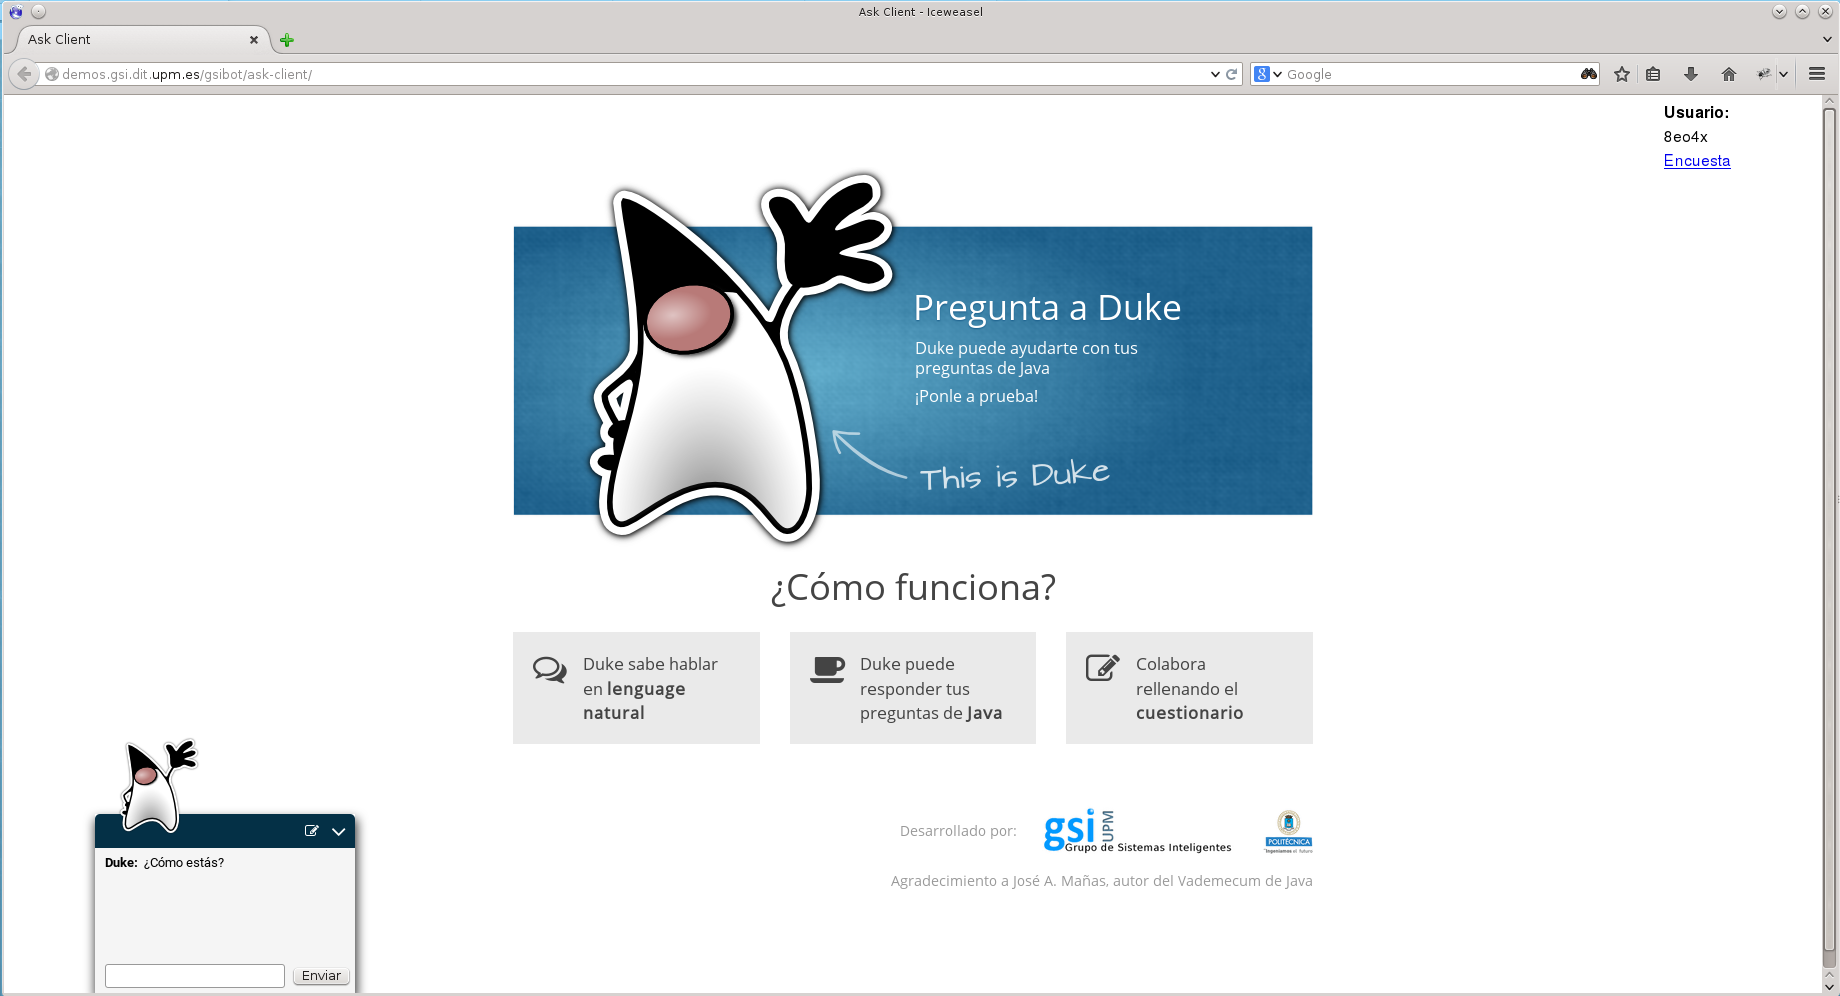
\includegraphics[width=0.7\textwidth]{img/screens/ask-client.png}
    \caption{Web interface for the client.}
    \label{fig:chat1}
\end{figure}

The client is made using web technologies: HTML, CSS and Javascript, and uses Ajax to communicate with the server sending the user questions and handling the response, waiting for the user to send a question and then making the request to the server, as shown in listing \ref{listing:formclient}.

%\emph{\textcolor{red}{Add example of JSON request? Add html code?}}

\begin{center}
  \lstinputlisting[language=JavaScript, caption=Ajax performing the request to the controller, label=listing:formclient, firstline=77, lastline=118]{code/prot/ask.js}
\end{center}

Upon the user submitting a question through the interface, the client will send a GET request to the controller, as described in section~\ref{sec:frontendcon}, and will receive a json response, containing the answer and the page to be shown to the user, if existent. An example response to que question ``¿Qué es un for?'' is shown in listing~\ref{listing:jsonchatresponse}.

\begin{center} 
  \begin{lstlisting}[language=json, caption=Example response for the chat client, label=listing:jsonchatresponse]
   {
     "answer": [
		"Esto es lo que s\u00e9 sobre for",
		"Si quieres, creo que bucles for degenerados tienen algo que ver con esto"
	       ],
     "definition": "Los bucles for se ejecutan un n\u00famero determinado de veces",
     "links": [
                "http://www.dit.upm.es/~pepe/libros/vademecum/topics/3.html",
                "http://www.dit.upm.es/~pepe/libros/vademecum/topics/139.html",
                "http://www.dit.upm.es/~pepe/libros/vademecum/topics/140.html",
                "http://www.dit.upm.es/~pepe/libros/vademecum/topics/141.html",
                "http://www.dit.upm.es/~pepe/libros/vademecum/topics/142.html",
                "http://www.dit.upm.es/~pepe/libros/vademecum/topics/143.html"
                ] ,
     "resource": "http://www.dit.upm.es/~pepe/libros/vademecum/topics/138.html"
   }  
  \end{lstlisting}
\end{center}

\subsection{Front end controller}
\label{sec:frontendcon}
The Front end controller is the main control module in our system. It handles the requests received from the client described in \ref{sec:chatclient}, and proceeds to triggers the required modules, as well as executing the \ac{OoB} commands received from each module. This module is provided as a web service, and therefore we have chosen Flask~\cite{flask0101} and Apache's mod\_wsgi~\cite{modwsgi} to deploy it. In the following subsections we will describe how it works as well as its work-flow structure.

\subsubsection{Functional Model}

The function of this module is returning the answer to the user, formed as JSON, by triggering the appropriate modules and reacting to their responses. To do so, it follows a process explained in the UML diagram shown in Figure \ref{fig:fe-model1}.

\begin{figure}[!htbp]
    \centering
    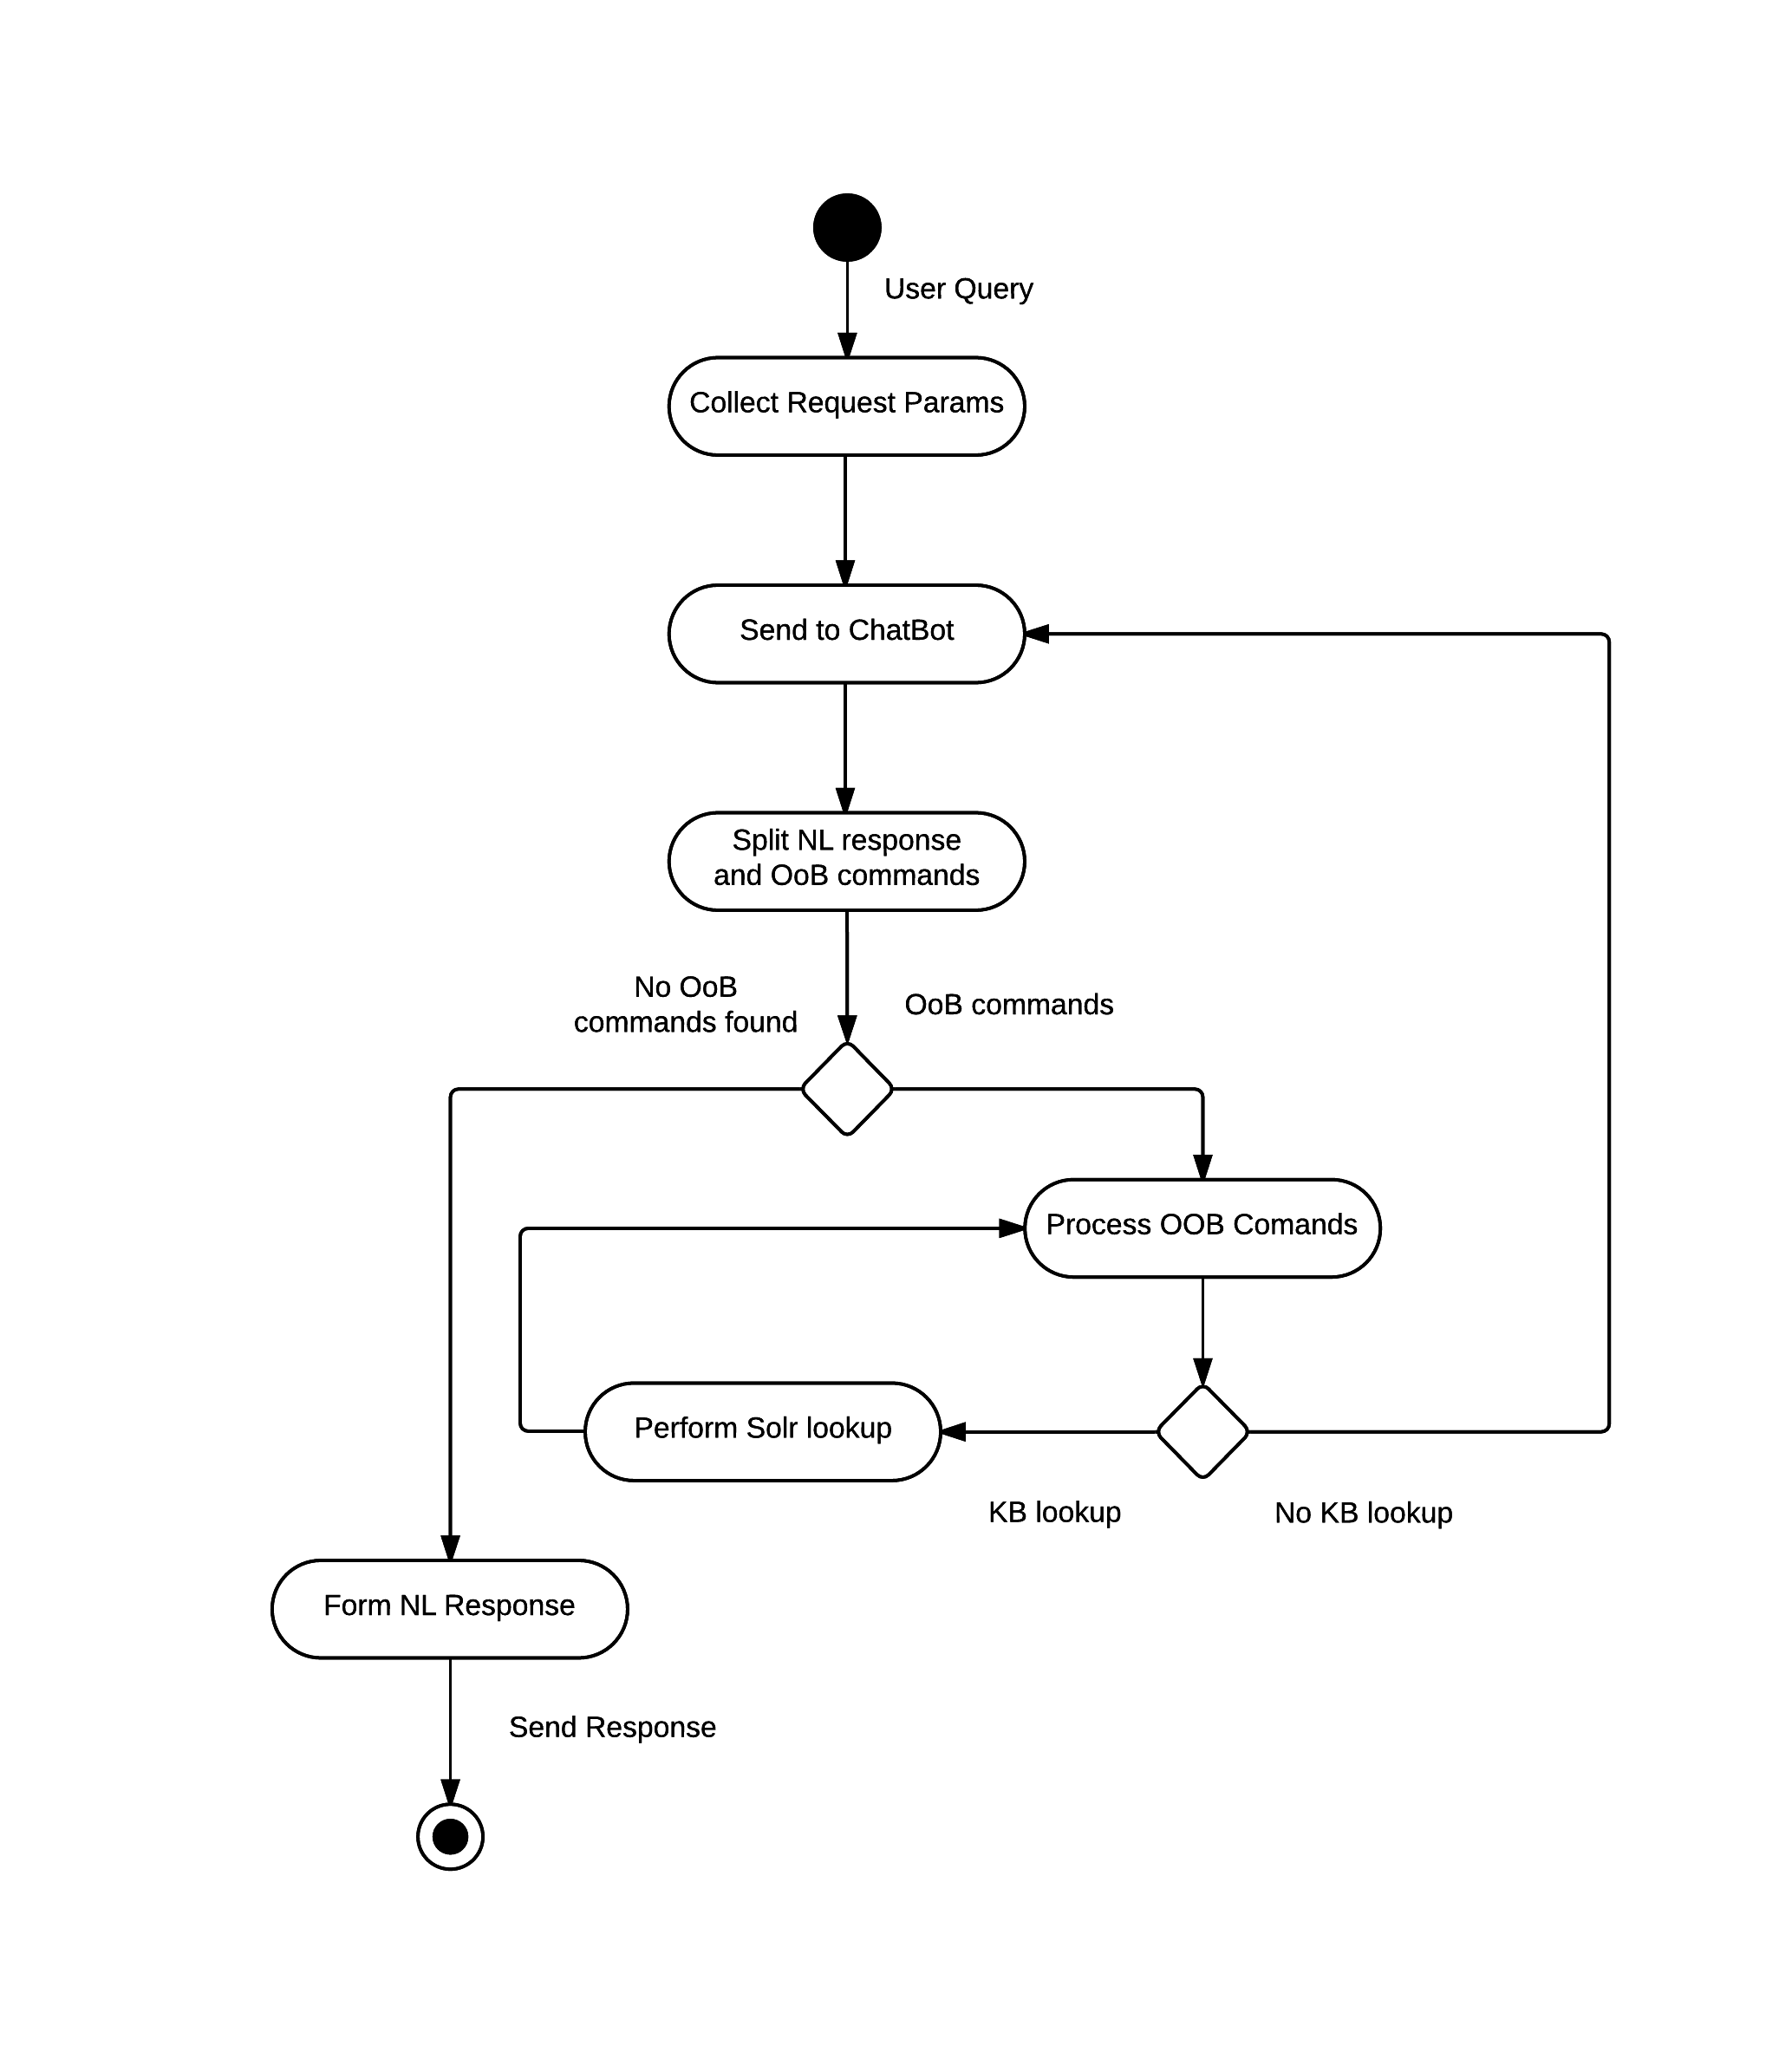
\includegraphics[width=0.8\textwidth]{img/prot/activityDiagram.png} 
    \caption{UML diagram of the process followed by the controller.}
    \label{fig:fe-model1}
\end{figure}

\begin{itemize}
 \item \textbf{Request parsing:} The client sends the query as JSON using a HTTP request to the front-end controller. This JSON is recovered and processed into a python dictionary.
 \item \textbf{Send to ChatBot:} The user query is sent to the ChatBot so it's processes and a response, either \ac{NL} or \ac{OoB}, is generated.
 \item \textbf{Split \ac{NL} response and \ac{OoB} commands} The response in the previous step is split in \ac{NL} and {OoB} commands, to process each one appropriately.
 \item \textbf{\ac{OoB} command processing:} Read the \ac{OoB} commands and take the appropriate steps for each one of them.
 \item \textbf{Solr Lookup:} If a lookup in the Knowledge base is required, send the query to Solr.
 \item \textbf{Form Response:} Once there are no more \ac{OoB} commands, form the actual response in JSON and send it to the user.
\end{itemize}

% Add the workflow of the controller.

\subsubsection{Structural Model}

In this section we will describe the structure followed designing the front end controller. In figure \ref{fig:fe-methods1} we show the method structure of the controller.
\begin{figure}[!htbp]
    \centering
    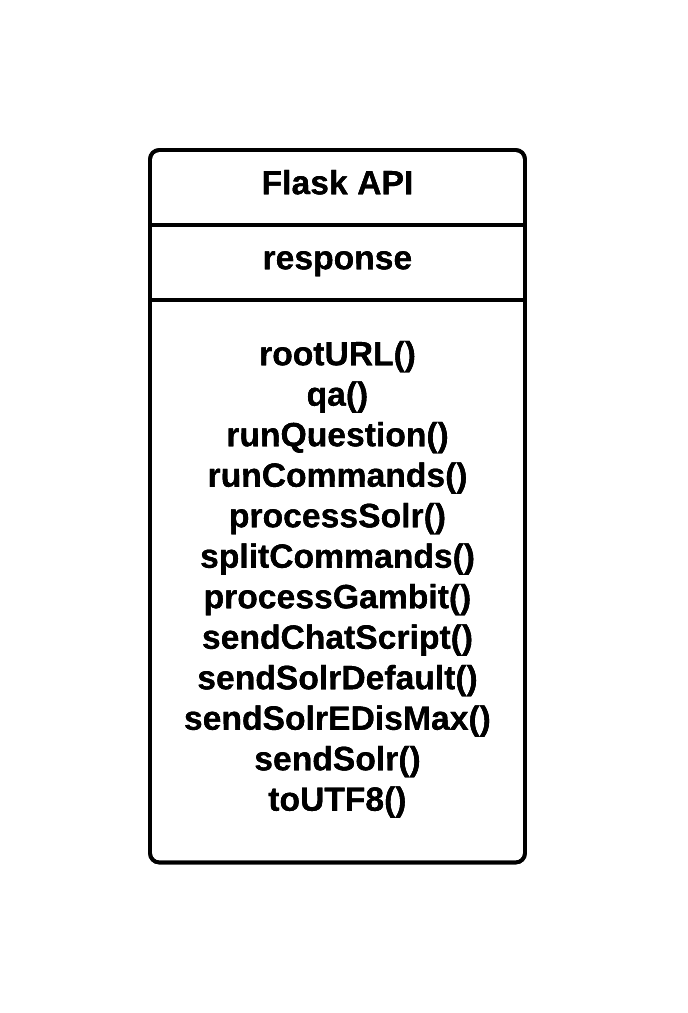
\includegraphics[width=0.4\textwidth]{img/prot/controllerStructure.png}
    \caption{Front end controller structure}
    \label{fig:fe-methods1}
\end{figure}

Now we will proceed to describe each of the methods shown in the figure.

\begin{itemize}
  \item \textbf{rootURL()} will be triggered whenever the base URL for the controller is requested. It will act in the same way than the qa() method.
  \item \textbf{qa()} this function will recover the request parameters, shown in table \ref{tab:fe-qparams}, and start the process to understand the user query, in order to return the appropriate response, whose parameters are shown on table \ref{tab:fe-rparams}.
  \item \textbf{runQuestion()} in this function, we will simply run the question once throught ChatScript, and then start the main command processing.
  \item \textbf{runCommands()} Given the \ac{NL} response from ChatScript, it will split the \ac{OoB} commands and start processing each one of them, as well as their responses, adding commands to the queue as needed.
  \item \textbf{processSolr()} For the solr command, this method will construct the solr query, and keep sending it to Solr increasing its fuzziness level, until an answer is found, or a maximum fuzziness is reached, in which case it will return the empty solr response.
  \item \textbf{splitCommands()} Taking a \ac{NL} sentence as a parameter, this method will return both a list with all the \ac{OoB} commands in the sentence, as well as the \ac{NL} part of the sentence, or an empty string if the sentence was made only of \ac{OoB} commands. 
  \item \textbf{processGambit()} when a direct search does not return any answer, the system will perform a broader search in Solr. This is further explained in section \ref{sec:solr}.
  \item \textbf{sendChatScript()} This function will process the interaction with ChatScript, both sending the questions and handling the responses. For more details, see section \ref{sec:chatbot}.
  \item \textbf{sendSolrDefault()} Given a question and no other parameters or information, this function will send said question to Solr, so it will go through the default processing. This is mainly unused.
  \item \textbf{sendSolrEDisMax()} When a gambit is needed, send the question to Solr using an \ac{eDisMax} query, which will search in different fields, valuing each field using a given weight. 
  \item \textbf{sendSolr()} Used by the rest of the Solr related methods, this function will handle sending the payload given as parameter to Solr, and returning the JSON response.
\end{itemize}

\begin{center}
  \begin{table}
    \begin{tabular*}{0.7\textwidth}{@{\extracolsep{\fill}} | c | c | p{0.5\textwidth} |}
      \hhline{|-|-|-|}
      \textbf{Parameter} & \textbf{Name} & \textbf{Description} \\ \hhline{|=|=|=|}
      question & User's question & The question submitted by the user. \\ \hhline{|-|-|-|}
      bot & Bot & The bot the query will be send to. \\ \hhline{|-|-|-|}
      username & The user & A random identifier for the user communicating with the bot. \\ \hhline{|-|-|-|}
      \end{tabular*}
    \caption{Parameters in the query received by the front end controller.}
    \label{tab:fe-qparams}
  \end{table}
\end{center}

\begin{center}
  \begin{table}
    \begin{tabular*}{0.7\textwidth}{@{\extracolsep{\fill}} | c | c | p{0.5\textwidth} |}
      \hhline{|-|-|-|}
      \textbf{Parameter} & \textbf{Name} & \textbf{Description} \\ \hhline{|=|=|=|}
      Answer & The Bot's response & The \ac{NL} response generated by the bot. \\ \hhline{|-|-|-|}
      Resource & An URL & The url of the relevant document where the information is, if existent. \\ \hhline{|-|-|-|}
      \end{tabular*}
    \caption{Parameters in the query sent back to the client.}
    \label{tab:fe-rparams}
  \end{table}
\end{center}

Finally, we will describe the \ac{OoB} commands that the system will be able to process.

\begin{itemize}
 \item \textbf{¬sendSolr} this command is issued whenever a question matches the pattern specified to request information about a Java topic.
 \item \textbf{¬solrResponse} after a search is performed in Solr, this command is issued to indicate whether or not a response has been found, and returning said response.
 \item \textbf{¬solrLinks} a special Solr search, looking for related topics in Solr.
 \item \textbf{¬solrLinksResponse} as a response to the solrLinks command, returns a list with the related topics.
 \item \textbf{¬gambit} perform an \ac{eDisMax} search in Solr, using the full user question.
 \item \textbf{¬gambitResponse} returns the title of the most relevant document found in the \ac{eDisMax} search.
 \item \textbf{¬gambitUnknown} issued when no document with a high enough score is found in Solr.
 \item \textbf{¬resource} sets the url to be displayed in the final response returned to the client.
 \item \textbf{¬label} sets the title of the found document as the label for the response.
\end{itemize}

The syntaxes of the commands is specified in table \ref{tab:oob-commands}.
\begin{center}
  \centering
  \begin{table}
    \begin{tabular*}{0.7\textwidth}{@{\extracolsep{\fill}} | c | c | p{0.35\textwidth} |}
      \hhline{|-|-|-|}
      \textbf{Command} & \textbf{Syntaxes} & \textbf{Description} \\ \hhline{|=|=|=|}
      ¬sendSolr & ¬sendSolr \textit{reqfield} \textit{doctitle} & Searchs in solr for the \textit{doctitle} and returns the \textit{reqfield} field.  \\ \hhline{|-|-|-|}
      \multirow{2}{*}{¬solrResponse} & ¬solrResponse \textit{unknown} & The requested document was not found in Solr. \\ \cline{2-3}
				     & ¬solrResponse \textit{reqfield} \textit{response} & Returns as \textit{response} the data of the field \textit{reqfield}. \\ \hhline{|-|-|-|}
      ¬solrLinks & ¬solrLinks \textit{linklist} & Asks for a search in Solr for the name of the topics given as an uri in the linklist \\ \hhline{|-|-|-|}
      ¬solrLinksResponse & ¬solrLinksResponse \textit{nameslist} & Sets the response for the ¬solrLinks command, returning the first name of the links. \\ \hhline{|-|-|-|}
      ¬gambit & ¬gambit \textit{topic}& Asks for a \ac{eDisMax} search on Solr, passing the full question. \\ \hhline{|-|-|-|}
      ¬gambitResponse & ¬gambitResponse \textit{gambittopic} & After performing an \ac{eDisMax} search, returns \textit{gambittopic} as the suggested topic. \\ \hhline{|-|-|-|}
      ¬gambitUnknown & ¬gambitUnknown & After performing an \ac{eDisMax} search, indicates that no relevant document has been found. \\ \hhline{|-|-|-|}
      ¬resource & ¬resource \textit{URL} & Sets \textit{URL} as the resource to be displayed in the client \\ \hhline{|-|-|-|}
      ¬label & ¬label \textit{topic} & Sets \textit{topic} as the concept of the response \\ \hhline{|-|-|-|}
      \end{tabular*}
    \caption{Parameters in the query sent back to the client.}
    \label{tab:oob-commands}
  \end{table}
\end{center}

\subsection{ChatBot}
\label{sec:chatbot}

The ChatBot handles the processing of the natural language input from the user, and controls the conversation. To do so, it uses the chat engine ChatScript, described in section \ref{subsec:chatscript}. We will first describe the ChatBot rules, and how they process the user input, and then proceed to describe how to launch and communicate with the ChatScript server.

\subsubsection{The rules}

Chatscript responds to a series of rules, specified in its topic files. This rules will match the user input and produce an appropriate response, or output a rejoinder if no rule is matched. A more in depth description of how chatscript rules work can be found in section \ref{subsec:chatscript}.

We have separated our topics across several files, each containing related topics, as well as the control script for the bot. We will start describing the control process, shown in listing~\ref{listing:cs-control}

\begin{center}
  \lstinputlisting[language=C++, captionpos=b, caption=Control process for ChatScript, label=listing:cs-control, firstline=16, lastline=80]{code/prot/control.top}
\end{center}

In this process, we first check if we are currently in any conversation and have any pending rejoinders ready to match the output. Then proceed to check for rules looking for matches in the JAVA and EJEMPLOS topics. If no answer is provided, we will look for gambits and proper responses in the current topic, and then in the rest of the topics with keywords associated. In the case no match have been found yet, the user input will be test against the keywordless topic, looking for both responses and gambits, and, finally, if there is still no response, a generic answer will be provided, asking the user to modify its question.

As we have just mentioned, there are several topics, both with and without keyword, spread across several files, containing both said topics and the sets of concepts used in the bot. This files and the topics contained in them are:

\begin{itemize}
 \item \textbf{topic.top} This file has most of the concepts used in the other files, as well as three generic topics:
 \begin{itemize}
  \item \emph{TENCUESTA} to answer questions regarding the poll that will be presented to the user.
  \item \emph{EXAMENES} containing generic responses to questions about the exams.
  \item \emph{INTRO} with information that will allow the bot to identify himself.
 \end{itemize}
 \item \textbf{java.top} This file contains the two main topics for answering the java questions.
 \begin{itemize}
  \item \emph{JAVA} will answer the questions related to java concepts, as well as produce gambits and question the user when the bot has the control over the conversation.
  \item \emph{EJEMPLOS} a slight variation from the previous topic, this will handle example requests from the user.
 \end{itemize}
 \item \textbf{javaconcepts.top} contains the list of all the java concepts that the bots knows about. It is automatically generated from the data stored in Solr.
 \item \textbf{insults.top} with the topic of the same name (INSULTOS), responds to insults and bad words input by the user.
 \item \textbf{estado.top} a single topic file, responsible of responding when the user enters information about himself, or asks the bot abouts its status.
\end{itemize}

All this files need to be compiled into binary data to be used by the ChatScript server.
% Explain how chatscript works.

\subsubsection{The server}

ChatScript provides two ways of interaction. For debugging purposes, it has a command line interface, and can also be deployed as a service listening in a TCP socket for user input. This server is what we have choose to use to interact with ChatScript. The full deployment instructions can be found in the appendix, and we will proceed to describe here the communication process.

As stated ChatScript listens on a TCP socket, waiting for requests containing three null separated strings, described in table~\ref{tab:cs-reqparams}

\begin{center}
  \centering
  \begin{table}
  \begin{center}
    \begin{tabular*}{0.6\textwidth}{@{\extracolsep{\fill}} | c | p{0.5\textwidth} |}
      \hhline{|-|-|}
      \textbf{Field} & \textbf{Description} \\ \hhline{|=|=|}
      user & The string identifying the user performing the question.  \\ \hhline{|-|-|}
      bot & The bot that the question is directed to, in case there are several bot available in the server. \\ \hhline{|-|-|}
      question & The user question \\ \hhline{|-|-|}
      \end{tabular*}
    \caption{Fields for the request to ChatScript}
    \label{tab:cs-reqparams}
    \end{center}
  \end{table}
\end{center}

The server will then return in the same connection the response generated using the process previously explained, and close the connection. If a new interaction is needed, a new socket will be opened, following the same process.
% \subsubsection{Using Spanish dictionaries}

%\emph{\textcolor{red}{It doesn't look viable to have spanish dicts in a timely manner.}}

\subsection{Solr instance}
\label{sec:solr}

In this section we will describe how the Solr instance is set up, as well as the schema and the search procedure. We are using Apache Solr 4.10.2 as a document and search engine. The search queries will be send by the controller described in section \ref{sec:frontendcon}. The server will contain the data recovered from the vademecum, structured in documents (one for each topic), and will allow us to perform the required searches. We will first describe the schema for the aforementioned documents, 

% Add the API rest for solr here?

% Add the relevant info from the sorlconfig here?

% Solr - add the relevant schema portions and how they work.

% Add somewhere how we are parsing the documents into json data.
\subsubsection{Data schema}
\label{subsec:solrschema}

The scrapped data is stored using a Solr core containing every relevant document. This is done by describing the structure of said documents in the schema.xml for Solr. In this file, we can consider three main groups of fields:

\begin{itemize}
 \item \textbf{Stock solr fields: } This fields are internal for solr, and we will not describe them here.
 \item \textbf{Document fields: } the fields scrapped from the Vademecum, they are described in table \ref{tab:schema-docfields}.
 \item \textbf{titleDefinition field: } this fields is generated concatenating the definition and title fields, to facilitate general search. %\emph{\textcolor{red}{Describe the copy process?}}

\end{itemize}

The xml for this fields is as in listing \ref{listing:solr-schema1}
\begin{center}
  \lstinputlisting[language=XML, captionpos=b, caption=fields defined for the java documents in the schema, label=listing:solr-schema1, firstline=125, lastline=148]{code/prot/schema.xml}
\end{center}

\begin{center}
  \centering
  \begin{table}
  \begin{center}
    \begin{tabular*}{0.655\textwidth}{@{\extracolsep{\fill}} | c | c | p{0.3\textwidth} |}
      \hhline{|-|-|-|}
      \textbf{Field} & \textbf{Field Type} & \textbf{Description} \\ \hhline{|=|=|=|}
      title & text\_search\_es & The title of this particular document.  \\ \hhline{|-|-|-|}
      alternative & lowercase & If exists, the English name for the document. \\ \hhline{|-|-|-|}
      concept & lowercase & What concept does this document refers to. \\ \hhline{|-|-|-|}
      resource & string & The link for this document. \\ \hhline{|-|-|-|}
      definition & text\_search\_es & The first sentence of the document. \\ \hhline{|-|-|-|}
      description & text\_search\_es & The text of the document. \\ \hhline{|-|-|-|}
      links & text\_ws & Related documents to this one. \\ \hhline{|-|-|-|}
      examples & text\_general & The scrapped text of the examples. \\ \hhline{|-|-|-|}
      \end{tabular*}
    \caption{Fields for the documents stored in the Solr schema.}
    \label{tab:schema-docfields}
    \end{center}
  \end{table}
\end{center}

As shown in the table, the fields have a ``field type'' associated, that will determine how they are stored and how they are tokenized and processed when performing the indexing and the search. The fieldTypes we are using are as follow:

\begin{itemize}
 \item \textbf{ string } This field is a default Solr field, and stored verbatim using the solr.StrField class.
 \item \textbf{ text\_general } A default Solr field, using the sorl.TextField class.
 \item \textbf{ lowercase } A variation on the default lowercase fieldType by Solr, it used the default keyword tokenizer and the lowercase filter, and we have added the ASCIIFolding filter.
 \item \textbf{ text\_search\_es } Based on Solr's Spanish fields, this field will contain general texr to perform a search. It uses a standard tokenizer, as well as the following filters:
 \begin{itemize}
  \item Lowercase filter: converts all words to lowercase 
  \item Stopfilter factory using Spanish stopwords and the snoball stemming algorithm
  \item Spanish light stem filter, a default solr stemmer for Spanish.
  \item Only for the query processing, a worddelimiter filter to do the QA.
 \end{itemize}
\end{itemize}

The listing \ref{listing:solr-schema2} shows the description of the text\_search\_es fieldType.

\begin{center}
  \lstinputlisting[language=XML, captionpos=b, caption=Definition for the text\_search\_es fieldType, label=listing:solr-schema2, firstline=542, lastline=567]{code/prot/schema.xml}
\end{center}

With this configuration we will be able to do the queries described in the following sections.

% Add something about the solr config?

\subsubsection{Faceted query}
% Maybe change the title?

In the event that ChatScript identifies the question and the topic the user is asking for, we will perform a faceted search in Solr, looking for the fields requested in the \ac{OoB} command. The query will be done in json format. An example of a query is shown in listing \ref{listing:solrquery1}, and the meaning of each field is described next:

\begin{center} 
  \begin{lstlisting}[language=json, caption=Example json query for Solr, label=listing:solrquery1]
   {
     "q" : "title:for~0",
     "wt" : "json",
     "fl" : "*,score",
     "rows" : "1"
   }  
  \end{lstlisting}
\end{center}

\begin{itemize}
 \item \textbf{q} contains the actual query sent to the server, specifying the fields we are looking for, as well as the expected filter for the query and the fuzziness. In the example, we are searching for documents containing the given string in the title, with a fuzziness of 0 (an exact match).
 \item \textbf{bf} the format the data will be returned in. In the example, we want the data in json format.
 \item \textbf{fl} the list of fields we want for the documents in the response. In the example, this is set to all the fields in the document, specified in the query as a wild card ``*'', as well as the score for the match.
 \item \textbf{rows} the number of documents to return.
\end{itemize}

With this search, we will try to look up the documents when the ChatScript module clearly identifies the topic the user is asking about, and, properly defining the returning fields for the search, the controller will show the relevant data. In case the question is not clearly identified, but ChatScript recognizes the user is talking about some java topic, this query won't be valid, and we will have to perform an \ac{eDisMax} query, described in the next section.

\subsubsection{Gambit query}
\label{subsec:solrgambit}
% Explain the process to run the eDisMax query

When ChatScript identifies a sentence talking about a java concept, but does not recognize a question, we will perform a search in Solr using the entire question, treating it as a \ac{QA} system. To do so, we will perform an \ac{eDisMax} query, taking advantage of the stemmers and tokenizers we have configured in section~\ref{subsec:solrschema}. This type of query is designed to process user input directly, searching for the keyword across multiple fields, with different boosts based on the significance of each field, and allowing multiple options to influence the score on a case to case basis.

Like the regular Solr query, this query is perform using a json format, and sent to the Solr service as the payload to a GET request. An example of an \ac{eDisMax} query is shown in listing \ref{listing:solrqueryeDisMax}

\begin{center} 
  \begin{lstlisting}[language=json, caption=Example \ac{eDisMax} query for Solr, label=listing:solrqueryeDisMax]
   {
     "q": "hablame de los bucles for",
     "defType": "edismax",
     "qf": "title^10.0 description^2.0",
     "fl": "*,score",
     "rows": "1",
     "wt": "json",
     "lowercaseOperators": "true",
     "stopwords": "true"
   }  
  \end{lstlisting}
\end{center}

The significance of each in the query is as follows:

\begin{itemize}
 \item \textbf{q} The question as sent by the user, with no processing.
 \item \textbf{defType} Explicitly set the query type as \ac{eDisMax}.
 \item \textbf{qf} Set the weights for each field to consider in the query.
 \item \textbf{fl} The fields to return.
 \item \textbf{rows} The number of documents to return.
 \item \textbf{wt} The format for the response.
 \item \textbf{lowercaseOperators} Interpret lowercase words as boolean operators, such as ``and'' and ``or''.
 \item \textbf{stopwords} Use the stopwords defined in the schema.
\end{itemize}

This search will provide a broader match than the faceted query, finding matches when the topic of the question is not clear, and offering the answer to the user. To prevent completely unrelated topics to be offered to the user, the score is retrieved and only the answers with a minimum score will be returned.


\subsection{Scrapping process}
% \emph{\textcolor{red}{Add a section describing the scrapped documents, and the rdf data?}}


% \section{Use cases}

% ¿? Something something... or something else?